\section{Swagger}{
		\begin{figure}
	\centering
	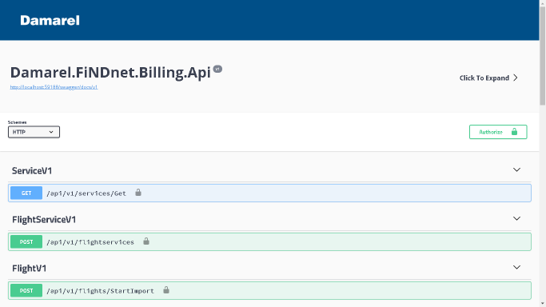
\includegraphics[width=\textwidth]{SwaggerUI}
	\caption{A Screenshot of the Swagger UI}
	\label{fig:SwaggerUI}
\end{figure}
	Before going on to describe the work I completed using Swagger, Firstly I shall explain what it is and how it can be used. Swagger is an API Description tool it allows for information about the endpoints of the API to be described. For example, it can state the formats of the inputs and outputs of the endpoint. The Swagger document is the file which contains all of the information on the API and is stored in the JSON format. This JSON file can then be parsed by a number of different programs to create interfaces which allow you to use/test the API. Alex my mentor set-up the Swashbuckle package in the API project. Swashbuckle is a tool which can generate a swagger document using the XML comments and some attributes from a C\# Web Project. Also, included in the swashbuckle release is the Swagger UI package. Swagger UI is a website which generates a testing ground for an API given a Swagger document input. Swagger have a test page which can be found at \url{http://petstore.swagger.io/} which can better demonstrate how it can be used. My job was to make some modifications to the Swagger document created by Swashbuckle and also to make some modifications to the Swagger UI to give it more of a Damarel theme. I learn quite a bit working on this project like how open source pieces of software are used in commercial environments. Also, I  did find a bug in the Swagger UI while working with it, therefore, I needed to submit a bug report to get it fixed. This introduced me to how Github works with their issues system.
}